\documentclass[]{article}
\usepackage[utf8]{inputenc}
\usepackage[pdftex]{graphicx} % for includegraphics
\usepackage[bf,font={small,sl}]{caption} % for pretty captions
\usepackage{natbib} % for the bibliography
\usepackage{amsmath} % for align and cases
\usepackage{listings} % for lstlisting
\usepackage{color} % for lstlisting background color

% listing style
\definecolor{lightgrey}{rgb}{0.95,0.95,0.95}
\lstset{
	backgroundcolor=\color{lightgrey},
	basicstyle=\footnotesize,
  	breakatwhitespace=false,
 	breaklines=true,
  	keepspaces=true,
  	language=R,
  	tabsize=2,
  	deletekeywords={data,step}
}

\title{\texttt{moveHMM}\\ An R package for animal movement modelling}
\author{Michelot T., Langrock R., Patterson T., and Rexstad E.}

\begin{document}
\maketitle

\section*{Introduction}
Animal movement data is growing rapidly, due to the substantial improvement of telemetry technologies. As a result, statistical methods used to analyse this data are brought to their computational limit.

Novel models have been developed in the last decade to reduce the computational cost of statistical inference in movement ecology. In particular, hidden Markov models are increasingly popular in this field, due to their flexibility, and to the efficient algorithms that they offer, see \cite{patterson2009} and \cite{langrock2012}.\\

\texttt{moveHMM} is an R package which implements hidden Markov models (HMMs) for animal movement. A special attention was paid to performance, and the fitting algorithm is implemented in C++ to make it significantly faster.

The goal of this vignette is to give a global overview of the possibilities offered by the package, and to demonstrate its use on a detailed example.

\section{Package features}
In this section, we describe different features included in \texttt{moveHMM}. We describe the global structure of the package, and then describe in more detail the main functions required to fit a HMM to movement data. In particular, we introduce the different options that the functions offer, and explain how the functions' arguments should be chosen.

\subsection{Structure}
The package is articulated around two S3 classes : \texttt{moveData} and \texttt{moveHMM}. The first one is a data frame of the data, essentially gathering time series of the movement metrics of interest, namely the step lengths and turning angles, as well as the covariate values. A \texttt{moveHMM} object is a fitted model, which stores in particular the values of the MLE of the parameters.\\

In order to create a \texttt{moveData} object, the function \texttt{prepData} is called on the tracking data (track points coordinates). Then, the function \texttt{fitHMM} is called on the \texttt{moveData}, and returns a \texttt{moveHMM}.

Both classes can be used through their methods, e.g. \texttt{plot.moveData}, \texttt{decode.moveHMM}, \texttt{AIC.moveHMM}... All the functions are described in more detail in Section \ref{main_functions}, and their use is explained on an example in Section \ref{application}.\\

Figure \ref{struct} illustrates the links between the main components of the package.

\begin{figure}[h]
	\centering
	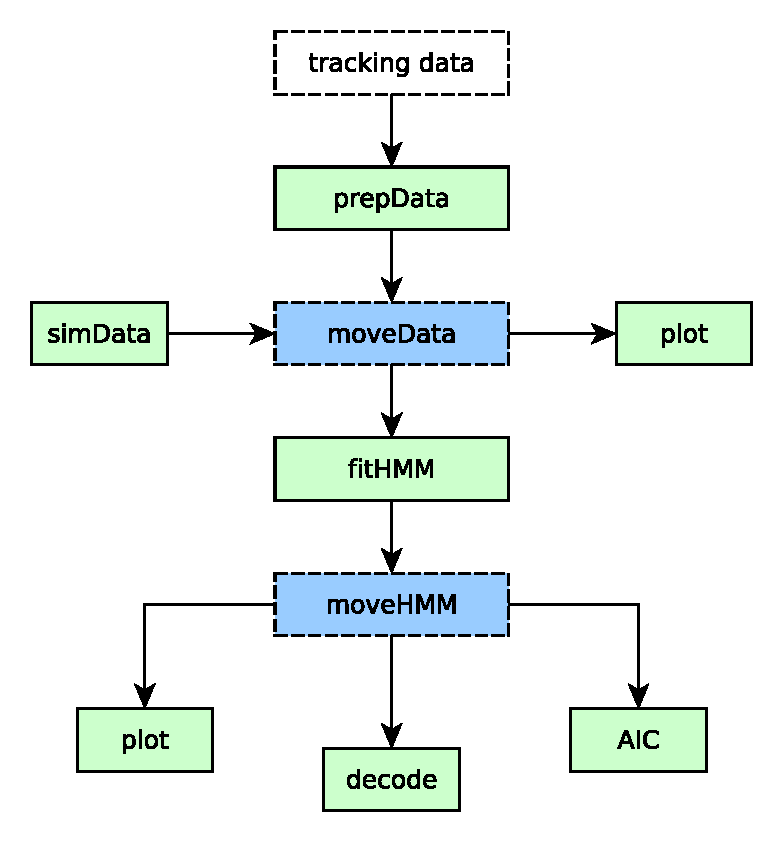
\includegraphics[width=0.5\textwidth]{pictures/struct}
	\caption{Structure of the main components of the package. The blue boxes are S3 classes, and the green boxes are functions. The arrows indicate input and output of data.}
	\label{struct}
\end{figure}

\subsection{Model options}

\subsubsection{Distributions}
Here is the list of distributions included, with the names they have in the package.
\begin{itemize}
	\item Step length : Gamma (``gamma''), Weibull (``weibull''), exponential (``exp''), and log-normal (``lnorm'').
	\item Turning angle : Von Mises (``vm''), and wrapped-Cauchy (``wrpcauchy''). It is also possible to specify \texttt{angleDist="none"}, if the angles should not be modelled.
\end{itemize}

The parameters depend on the distribution used. The Gamma distribution expects the mean and standard deviation, and all other distributions expect the same parameters as the corresponding R density function, i.e.
\begin{center}
\begin{tabular}{lcll}
	Distribution & & Parameters & \\
	\hline
	Gamma & & mean & standard deviation\\
	Weibull & & shape & scale\\
	Log-normal & & log-mean & log-standard deviation\\
	Exponential & & rate & \\
	\hline
	Von Mises & & mean & concentration\\
	Wrapped Cauchy & & mean & concentration\\
	\hline	
\end{tabular}
\end{center}

For the Gamma distribution, the link between the mean/standard deviation (expected by \texttt{fitHMM}) and scale/rate (expected by \texttt{dgamma}) is given by :
\begin{align*}
	scale & = \dfrac{(mean)^2}{(sd)^2}\\
	rate & = \dfrac{(mean)^2}{sd}
\end{align*}

\subsubsection{Zero-inflation}
It is possible to inflate the step length distribution at $0$, by specifying \texttt{zeroInflation=TRUE} in \texttt{fitHMM}. Zero-inflation can be defined as follows.\\

Let $X_t$ be the random variable of the step length of the animal at time $t$. Let $\mathcal{D}(\theta)$ be the distribution of $X_t$, and $z \in [0,1]$ its inflation in $0$. Then,

\begin{equation*}
	\begin{cases}
		X_t = 0 \text{ with probability $z$}\\
		X_t \sim \mathcal{D}(\theta) \text{ with probability $1-z$}
	\end{cases}
\end{equation*}

In the package, the distribution $\mathcal{D}$ will be one of the Gamma, Weibull, log-normal or exponential distributions.

\subsubsection{Covariates}
It is possible to model the state transition probabilities as functions of time-varying covariates. To do so, an additional parameter is included in the model, \texttt{beta}. This matrix contains the coefficients of the multinomial logistic regression which links the covariate values to the transition probabilities.\\

Let $(C_t)$ be the state process, and $\gamma_{ij} = \Pr(C_{t+1}=j \vert C_t=i)$. Then, 

\begin{equation*}
	\gamma_{ij}(t) = \dfrac{\exp\left(\beta_0^{(ij)} + \sum_k \beta_k^{(ij)} x_k(t)\right)}{1+\exp\left(\beta_0^{(ij)} + \sum_k \beta_k^{(ij)} x_k(t)\right)}
\end{equation*}

where the $x_k$ are the different covariates.\\

In addition, we consider the following constraint on the row sums of the transition probability matrix :
\begin{equation*}
	\forall t, \forall i, \sum_j \gamma_{ij}(t) = 1
\end{equation*}

This implies a constraint on the $\beta_k^{(ij)}$ coefficients. If $n$ is the number of states of the HMM, then only $n(n-1)$ coefficients are required, for each covariate, to deduce the corresponding transition probabilities.

In practice, we chose to store coefficients for the non-diagonal transition probabilities. For example, for a 3-state HMM with two covariate, the matrix \texttt{beta} is,
\begin{equation*}
	\beta =
	\begin{pmatrix}
	\beta_0^{(12)} & \beta_0^{(13)} & \beta_0^{(21)} & \beta_0^{(23)} & \beta_0^{(31)} & \beta_0^{(32)}\\
	\beta_1^{(12)} & \beta_1^{(13)} & \beta_1^{(21)} & \beta_1^{(23)} & \beta_1^{(31)} & \beta_1^{(32)}\\
	\beta_2^{(12)} & \beta_2^{(13)} & \beta_2^{(21)} & \beta_2^{(23)} & \beta_2^{(31)} & \beta_2^{(32)}\\		
	\end{pmatrix}
\end{equation*}

\subsubsection{Stationarity}
\textit{Ask Roland to write this.}

\subsection{Main functions} \label{main_functions}

\subsubsection{prepData}
Most of the time, tracking data consists in time series of either easting-northing coordinates or longitude-latitude values. However, the data needed to use hidden Markov modelling are the time series of step lengths and turning angles.\\

The function \texttt{prepData} computes the steps/angles from the coordinates. As an input, this function takes an R data frame with mandatory column names ``x'' (either easting or longitude) and ``y'' (either northing or latitude). If several animals were observed, there should also be a colum ``ID'' which identifies the animal being observed. If there is no ``ID'' column, all observations will be considered to concern a single animal. All additional columns are considered as covariates.

In addition to the data frame, \texttt{prepData} takes an argument \texttt{type}, which can either be ``GCD'' (default) or ``euclidean''. The former indicates that the coordinates are longitude-latitude values, and the latter that they are easting-northing values. This option is used in the computation of the step lengths.

To do so, \texttt{prepData} calls the function \texttt{spDistN1}, from the package \texttt{sp}. The step lengths are in the metrics of the input if easting/northing are provided, and in kilometres if longitude/latitude are provided.\\

\texttt{prepData} outputs a data frame, with the same columns as the input, plus columns ``step'' and ``angle''. This object is of the class \texttt{moveData}, and can be plotted using the generic method \texttt{plot}.

\subsubsection{fitHMM}
To an object \texttt{moveData} can then be fitted an HMM, using the function \texttt{fitHMM}. The list of its arguments is detailed in the documentation.

The maximum likelihood estimation is carried out using the R function \texttt{nlm}.\\

This function outputs a list of information about the model. Most elements of that list are only meant to be used by the \texttt{moveHMM} methods (see Section \ref{methods}), but a few can be informative \textit{per se} :
\begin{itemize}
	\item \texttt{mle} contains the estimates of the parameters of the model;
	\item \texttt{mod} contains the output of the optimization function \texttt{nlm}, including \texttt{mod\$minimum} (minimum of the negative log-likelihood) and \texttt{mod\$hessian}, the hessian of the negative log-likelihood function at its minimum.
	\item \texttt{states} contains the sequence of most probable states, as computed by the Viterbi algorithm \citep{zucchini2009}.
\end{itemize}

\subsubsection{Classes methods} \label{methods}
Methods (i.e. class functions) are available for both \texttt{moveData} and \texttt{moveHMM} objects, to operate on them. Here is a list of them ; for details on the options, see the documentation, and for an example of their use, see Section \ref{application}.

\begin{itemize}
	\item \texttt{plot.moveData} plots a few graphs to illustrate the data : a map of each animal's track, time series of the steps and angles, histograms of the steps and angles.
	\item \texttt{plot.moveHMM} plots a few graphs to illustrate the fitted model : a map of each animal's track, colored by states, plots of the estimated density functions, plots of the transition probabilities as functions of the covariates.
	\item \texttt{AIC.moveHMM} returns the AIC of the fitted model.
	\item \texttt{pseudoRes.moveHMM} computes the pseudo-residuals of the model.
	\item \texttt{stateProbs.moveHMM} computes the state probabilities for each observation.
	\item \texttt{decode.moveHMM} wraps \texttt{pseudoRes} and \texttt{stateProbs}.
	\item \texttt{confIntervals.moveHMM} computes the confidence intervals for the step length distribution parameters and for the regression coefficients of the transition probabilities.
	\item \texttt{deltaMethod.moveHMM} computes the confidence intervals for the turning angle distribution parameters, using the delta method.
\end{itemize} 

\subsubsection{simData}
The function \texttt{simData} simulates movement data from an HMM, given its parameters. The returned object is of the class \texttt{moveData}, and can then be visualized using \texttt{plot.moveData}, or fitted using \texttt{fitHMM}.

The arguments of \texttt{simData} are detailed in the documentation.

\section{Application} \label{application}
In this section, we illustrate the possibilities of the package on a real data example. We use the data from \cite{morales2004}, collected on four elks in Canada. 

\subsection{Movement data}
In order to be preprocessed and fitted, the data needs to have the correct format. It needs to be a \texttt{data.frame}, with two mandatory columns :
\begin{itemize}
	\item Easting or longitude (default name : \texttt{x})
	\item Northing or latitude (default name : \texttt{y})
\end{itemize}
It is possible to have a column ``ID'', which contains the identifiers of the observed animals. If no column named ``ID'' is provided, all the observations will be considered to concern a single animal.

Additional columns are considered as covariates. Note that covariates need to have numerical values.\\

\subsubsection{Load and format the tracking data}

The data is available from the following URL : 
\begin{center}
	http://www.esapubs.org/archive/ecol/E085/072/elk\_data.txt
\end{center}
We load the relevant rows and columns into a data frame using the \texttt{read.table} command.

\begin{lstlisting}
trackData <- read.table(
		"http://www.esapubs.org/archive/ecol/E085/072/elk_data.txt",
		sep="\t",header=TRUE)[1:735,c(1,2,3)]
\end{lstlisting}

The dataframe \texttt{trackData} now has three columns : ``Individual'', ``Easting'', and ``Northing''.

\begin{lstlisting}
> head(trackData)
  Individual Easting Northing
1    elk-115  769928  4992847
2    elk-115  766875  4997444
3    elk-115  765949  4998516
4    elk-115  765938  4998276
5    elk-115  766275  4998005
6    elk-115  766368  4998051
\end{lstlisting}

The animals' identifiers need to be stored in a column named ``ID'', before we can preprocess the data. Thus, we modify it accordingly.

\begin{lstlisting}
colnames(trackData)[1] <- "ID"
\end{lstlisting}

\subsubsection{Use \texttt{prepData}}
Now that the data has the right format, it is possible to call the preprocessing function \texttt{prepData}. We choose the arguments carefully :
\begin{itemize}
	\item \texttt{type} specifies whether the coordinates are easting/northing or longitude/latitude values. The latter is the default, so we need to call the function with the argument \texttt{type="euclidean"}, to indicate that we want to use the euclidean distance.
	\item \texttt{coordNames} are the names of the coordinates in the input dataframe. The default is ``x'' and ``y'', so we need to call the function with the argument \texttt{coordNames=c("Easting","Northing")}.
\end{itemize}

\noindent Eventually, the call to the function is,

\begin{lstlisting}
data <- prepData(trackData,type="euclidean",coordNames=c("Easting","Northing"))
\end{lstlisting}

The step lengths and turning angles are computed, and the returned object is a data frame.

\begin{lstlisting}
> head(data)
       ID      step      angle      x       y
1 elk-115        NA         NA 769928 4992847
2 elk-115 5518.4434  0.1262112 766875 4997444
3 elk-115 1416.5663  2.3832412 765949 4998516
4 elk-115  239.7525  0.9385238 765938 4998276
5 elk-115  432.7600  1.1375066 766275 4998005
6 elk-115  103.7545 -0.9687435 766368 4998051
\end{lstlisting}

Note that the coordinate have been renamed ``x'' and ``y''. This makes the processing of the data simpler.\\

If the data contains covariates, which have missing values, those are replaced by the closer non-missing value (by default, the previous one if it is available). This is arbitrary, and might result in misinterpretation of the data.

\subsubsection{Use \texttt{plot.moveData}}
Once the data has been preprocessed, it is possible to plot it, using the generic function \texttt{plot}. It displays maps of the animals' tracks, times series of the steps and angles, and histograms of the steps and angles. A few plotting options are available, and described in the documentation.\\

\noindent We want to plot all animals' tracks on a single map, so we call :

\begin{lstlisting}
plot(data,compact=T)
\end{lstlisting}

The resulting map, and the steps and angles graphs for the first animal, are displayed in Figure \ref{moveData}.

\begin{figure}[h]
	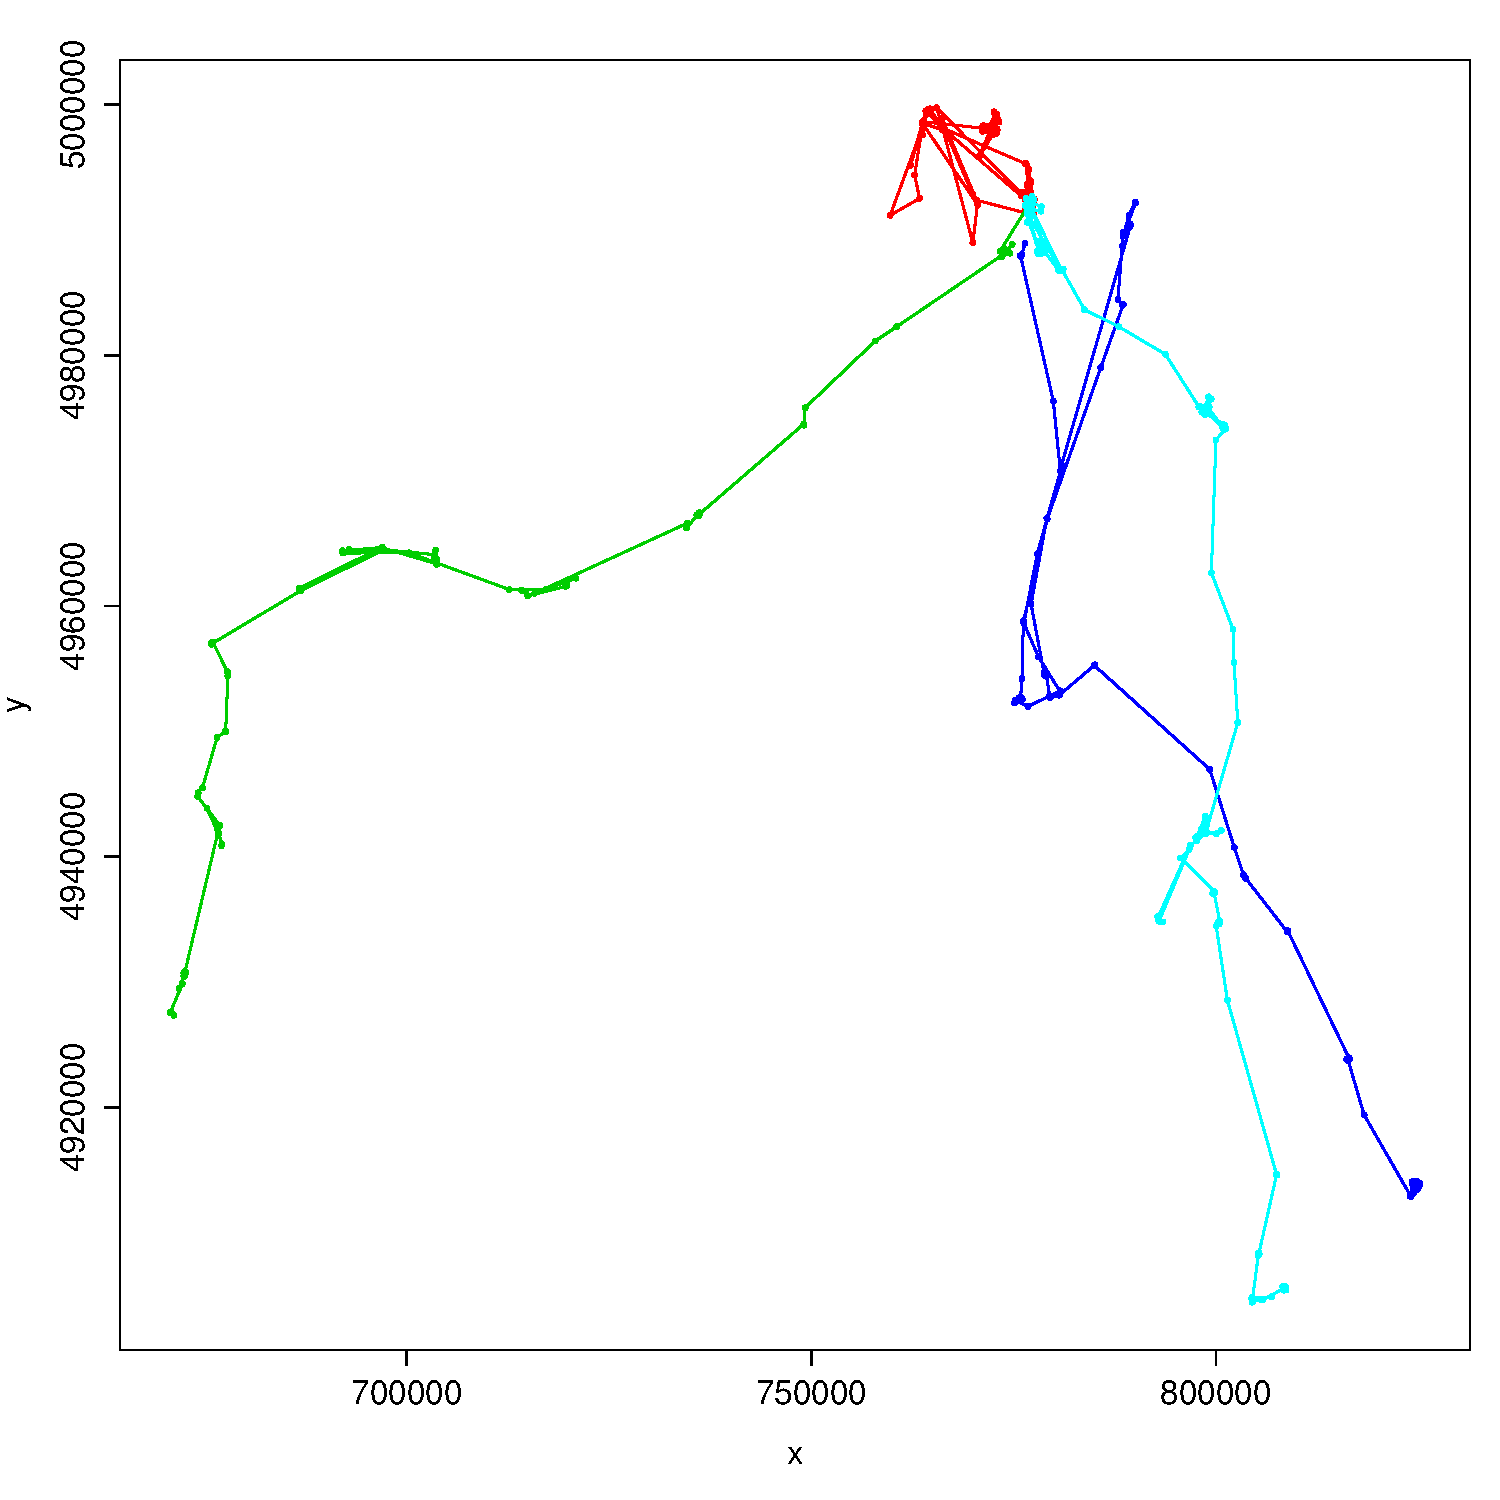
\includegraphics[width=0.49\textwidth]{pictures/map_moveData}
	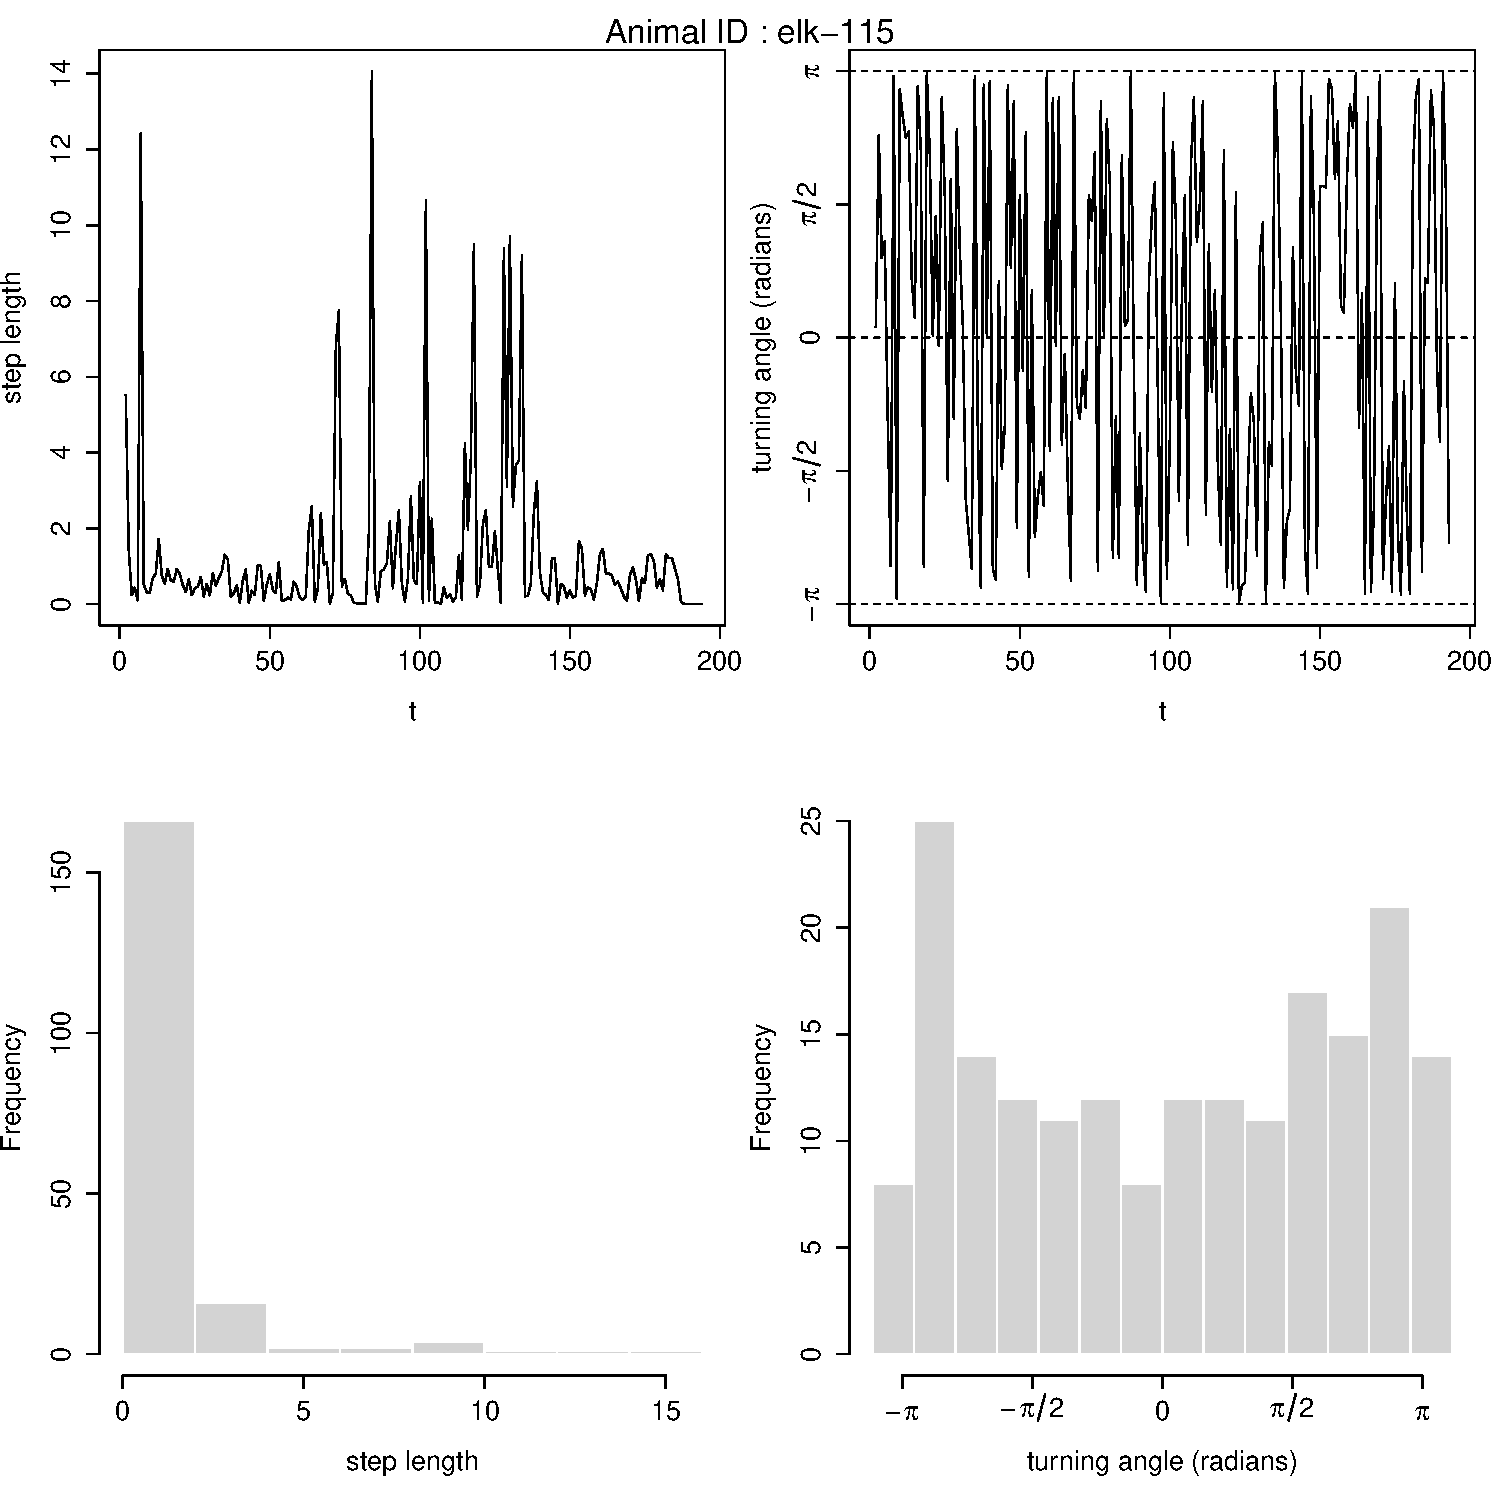
\includegraphics[width=0.49\textwidth]{pictures/graphs_elk1}
	\caption{Map of the animals' tracks (left) -- each color represents an animal. Graphs of the step lengths and turning angles for one individual (right).}
	\label{moveData}
\end{figure}

\subsection{Fitting the model}
We go through all the options of \texttt{fitHMM}, and demonstrate its use on the real data example.

Here we can warn the user about the choice of the initial values.

\subsection{Using the model}
We need to mention :
\begin{itemize}
	\item Plotting : describe the function \texttt{plot.moveHMM} and the graphical options, and display all the plots;
	\item Decoding : describe the decoding functions, such as \texttt{viterbi}, \texttt{stateProbs}, and \texttt{pseudoRes}, and apply them to the data;
	\item Assessing : we don't really have the functions yet, but we will need to explain how to obtain confidence intervals, and how to plot them. We might want to mention the simulation function as an assessing tool.
\end{itemize}


\begin{thebibliography}{}

\bibitem[\protect\citeauthoryear{Langrock et al.}{2012}]{langrock2012}
\textsc{Langrock R., King R., Matthiopoulos J., Thomas L., Fortin D., Morales J.M.} (2012),
``Flexible and practical modeling of animal telemetry data: hidden Markov models and extensions''
\textit{Ecology}, 93 (11), 2336--2342.

\bibitem[\protect\citeauthoryear{Morales et al.}{2004}]{morales2004}
\textsc{Morales, J.M., Haydon, D.T., Frair, J., Holsinger, K.E., Fryxell, J.M.} (2004),
``Extracting more out of relocation data : building movement models as mixtures of random walks'',
\textit{Ecology}, 85 (9), 2436--2445.

\bibitem[\protect\citeauthoryear{Patterson et al.}{2009}]{patterson2009}
\textsc{Patterson T.A., Basson M., Bravington M.V., Gunn J.S.} (2009),
``Classifying movement behaviour in relation to environmental conditions using hidden Markov models''
\textit{Journal of Animal Ecology}, 78 (6), 1113--1123.

\bibitem[\protect\citeauthoryear{Zucchini and MacDonald}{2009}]{zucchini2009}
\textsc{Zucchini, W.\ and MacDonald, I.L.} (2009).
{\em Hidden Markov Models for Time Series: An Introduction Using R.}
Chapman \& Hall (London).

\end{thebibliography}

\end{document}